Pre vytvorenie aplikácie, ktorá bude spĺňať požiadavky širokej škály užívateľov
a bude obsahovať prakticky využiteľné funkcie je potrebné spraviť prieskum existujúcich riešení
rovnako zameraných aplikácií dostupných na GooglePlay (pre Android) a iTunes (iOS).
Nižšie je uvedený zoznam najsťahovanejších mobilných aplikácií pre jednotlivé OS, ich funkcie, výhody,
nevýhody a chyby z užívateľského hľadiska.

\subsection*{Android}

\begin{description}
    \item [HDR Max - Photo Editor] (hodnotenie užívateľov 4.3/5)
    Na vytvorenie fotografie využíva natívnu aplikáciu Fotoaparát. Pri jednom spustení sa to ukázalo ako
    nevhodný spôsob, keďže sa po vytvorení fotografie neotvorila znova aplikácia. HDR fotografiu vytvára 
    pomocou filtra aplikovaného na jednu fotografiu. Filter sa dá dokonca kombináciou s inými krokmi naniesť 
    viac krát, čo sa dá považovať za chybu. Upravovanie HDR je veľmi obmedzené. Aplikácia obsahuje štandardné 
    úpravy vytvorenej fotografie (kontrast, jas, sýtosť, teplota a vyváženie farieb) a statické farebné filtre
    (obr. \ref{fig:appsUI_1}). Okrem toho má aplikácia ešte širokú ponuku, niekedy zbytočných funkcií.

    \item [Ultimate HDR Camera] (4.11/5)
    Fotografia sa vytvára v rozhraní aplikácie. Pre vytvorenie HDR formátu využíva kombináciu viacero vytvorených
    fotografií s rôzným expozičným časom. Následne vytvorená HDR fotografia má obmedzené úpravy. Aplikácia je
    veľmi jednoduchá, ale užívateľa nezaujme svojím rozhraním (obr. \ref{fig:appsUI_2}). Napriek tomu, výsledné snímky
    sú kvalitné zobrazenia scény s akýmkoľvek dynamickým rozsahom.

    \item [Snapseed] (4.5/5)
    Vytvorenie fotografie nie je možné, aplikácia dokáže iba načítať uloženú fotografiu z galérie, na ktorú je
    možné aplikovať filter, ktorý vytvára HDR efekt. Aplikácia však zaujala svojou ponukou grafických nástrojov,
    z ktorých najzaujímavejšie sú napr. nastavenie kriviek, perspektívy, retro filtre, rozpoznávanie tváre
    a efekt zostrenia (obr. \ref{fig:appsUI_3}). Aplikácia taktiež ponúka niekoľko málo farebných filtrov. Roz-hranie
    je intuitívne, a veľmi dobre premyslené vzhľadom na komplikované nástroje a možnosti úprav. Nastavovanie intenzity
    jednotlivých filtrov a úprav je zaujímavo implementované - pre výber nástroja využíva potiahnutie prstom vertikálne
    a potiahnutím prstom do strán nastavujeme intenzitu úpravy. Z pohľadu užívateľa je to najzaujímavejšia aplikácia
    na GooglePlay.

    \item [HDR Camera] (3.8/5)
    Fotografia sa vytvára v rozhraní aplikácie. Aplikácia vytvorí tri fotografie s rôznou expozíciou, čo trvá
    približne 5 sekúnd. Aplikácia je jedna z mála, ktorá nepoužíva na vytvorenie HDR filter. Po vytvorení HDR
    fotografie, nemá užívateľ žiadne ďalšie možnosti úprav. Užívateľ musí dostatočne rýchlo uložiť svoju výslednú
    fotografiu, pretože aplikácia sa svojvoľne prepína naspäť na domovskú obrazovku.

    \item [HDR HQ] (3.9/5)
    HDR fotografiu vytvára pomocou filtra aplikovaného na jednu vytvorenú fotografiu. Obsahuje obmedzené úpravy
    vytvorenej fotografie (kontrast, jas, teplota farieb). Užívateľa však zaujme jednoduché a minimalistické
    rozhranie aplikácie (obr. \ref{fig:appsUI_4}). Dôležitý nedostatok je však chýbajúce tlačidlo pre návrat
    z obrazovky úprav do hlavného menu.

    \item [A Better Camera] (4.1/5)
    Aplikácia obsahuje rôzne možnosti fotografovania scény, medzi ktorými je aj možnosť vytvorenia HDR fotografie.
    HDR fotografiu vytvára pomocou troch fotografií s rôznou expozíciou a výsledok je pre užívateľa dostatočne uspokojivý.
    Vytvorenú fotografiu je možne upravovať pomocou externej aplikácie od rovnakého vývojára.

\end{description}

\subsection*{iOS}

\begin{description}
    \item [HDR]
    HDR efekt vytvára pomocou jedného z piatich filtrov a nastavením jeho intenzity. Rozhranie je jednoduché
    a pre užívateľa nezaujímavé.

    \item [HDR Camera]
    Aplikácia je totožná s Android aplikáciou HDR HQ, čo pridáva pozitívnu vlastnosť - multiplatformnosť.
    Obdobne teda ako HDR HQ na Androide má veľmi zaujímave grafické rozhranie a zaujímavú ponuku úprav fotografie.

    \item [HDR for Free]
    Vytvorenie fotografie nie je možné, aplikácia dokáže iba načítať uloženú fotografiu z galérie, na ktorú je
    možné aplikovať jeden zo štyroch filtrov vytvárajúcich HDR efekt. Výsledok je aj tak veľmi neuspokojivý - iba
    sa zvýši kontrast farieb. Grafické rozhranie aplikácie je veľmi chabé.

    \item [Live HDR Camera]
    Fotografia sa vytvára v rozhraní aplikácie, kde užívateľ môže v reál-nom čase sledovať výsledok pomocou filtra
    obrazu. Obraz však obsahuje množstvo šumu a po vytvorení fotografie užívateľ dostane fotografiu upravenú filtrom
    s množstvom šumu. Po vytvorení fotografie aplikácia neponúka žiadne ďalšie nastavenia a~úpravy fotografie.

    \item [Snapseed]
    Aplikácia obsahuje všetky možnosti úprav a nástrojov ako Android aplikácia Snapseed.

    \item [Adobe Lightroom]
    Fotografia sa vytvára v rozhraní aplikácie, kde užívateľ môže nastavovať EV. HDR fotografiu následne vytvorí pomocou
    filtra. Užívateľovi ponúka štandardné úpravy a nastavenia, avšak rozhranie je veľmi ťažkopádne a neprehľadné.

\end{description}

\begin{figure}[t]
    \centering
    \begin{subfigure}{0.4\textwidth}
        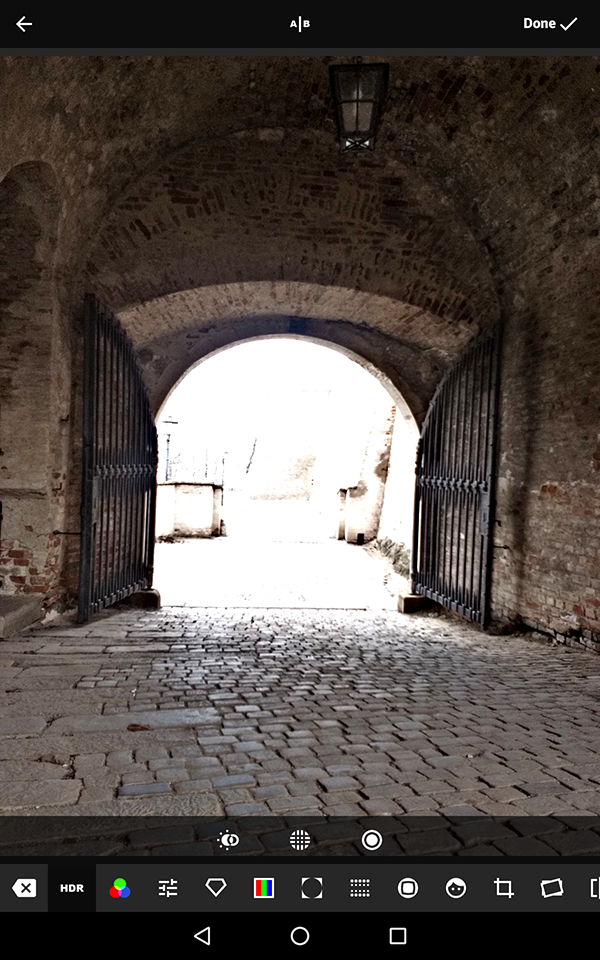
\includegraphics[width=\textwidth]{figures/ui/apps/uiHdrMax}
        \caption{HDR Max}
        \label{fig:appsUI_3}
    \end{subfigure}
    ~
    \begin{subfigure}{0.4\textwidth}
        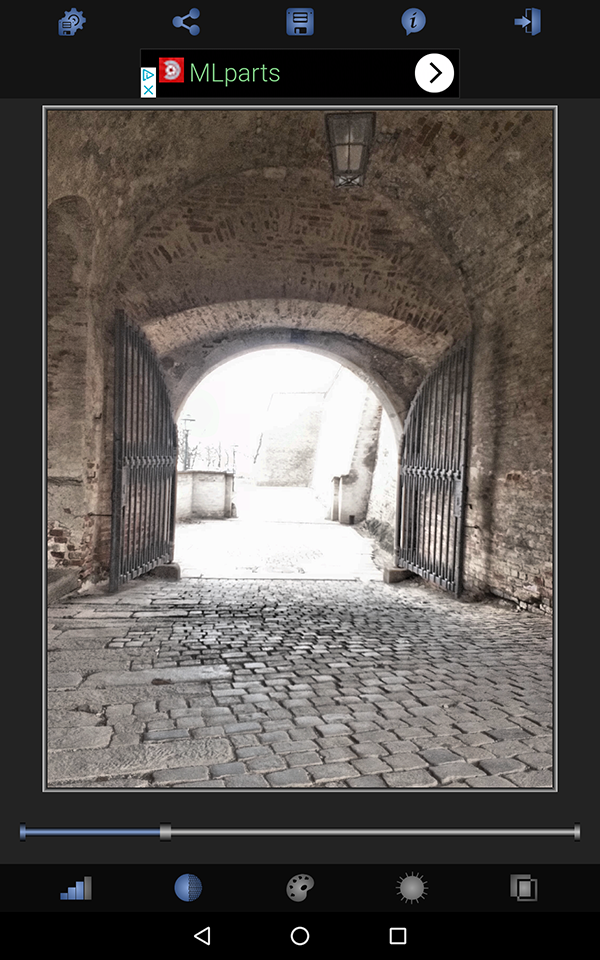
\includegraphics[width=\textwidth]{figures/ui/apps/uiUltimateHdr}
        \caption{Ultimate HDR Camera}
        \label{fig:appsUI_4}
    \end{subfigure}

    \begin{subfigure}{0.4\textwidth}
        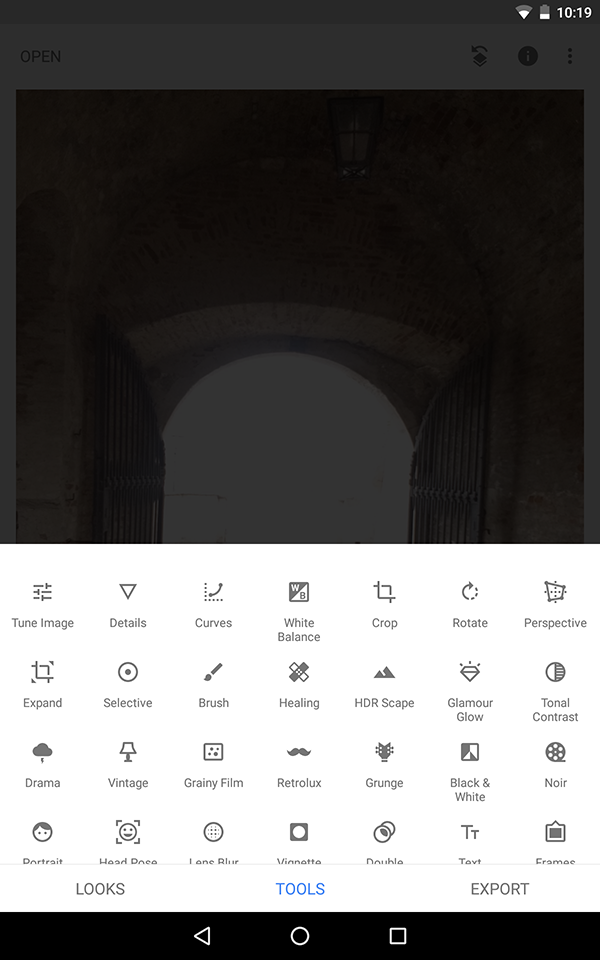
\includegraphics[width=\textwidth]{figures/ui/apps/uiSnapseed}
        \caption{Snapseed}
        \label{fig:appsUI_1}
    \end{subfigure}
    ~
    \begin{subfigure}{0.4\textwidth}
        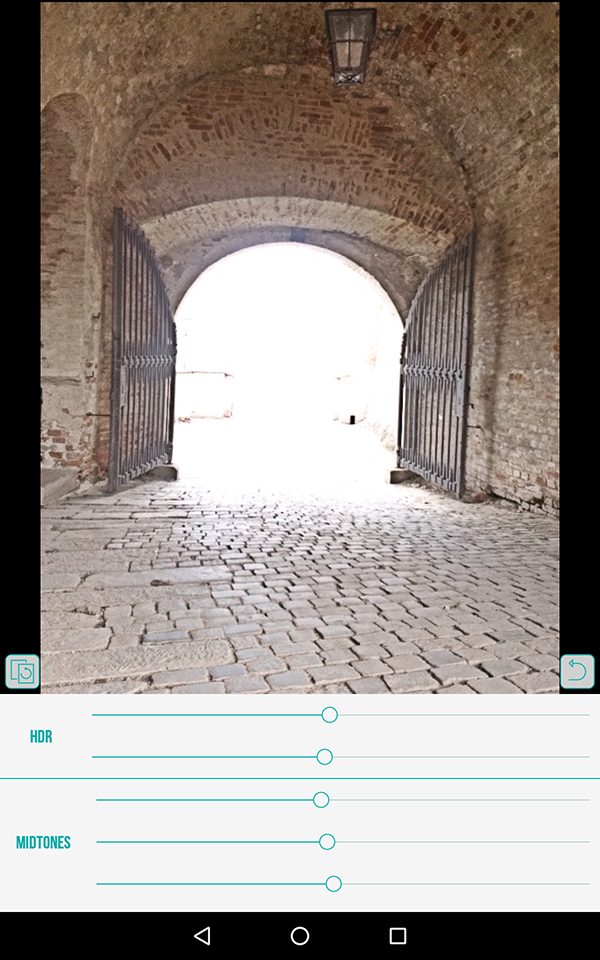
\includegraphics[width=\textwidth]{figures/ui/apps/uiHdrHq}
        \caption{HDR HQ}
        \label{fig:appsUI_2}
    \end{subfigure}
    \caption{Užívateľské rozhrania podobných aplikácií}
    \label{fig:appsUI}
  \end{figure}